\documentclass[11pt]{article}
\usepackage{fullpage}
\usepackage{listings}
\usepackage{needspace}
\usepackage{color}
\usepackage{ifthen}
\usepackage{pgf}
\usepackage{tikz}
\usetikzlibrary{arrows,automata}
\usepackage{amsmath}
\usepackage{url}
\usepackage{framed}
\usepackage{enumerate}
\usepackage{csc}
\usepackage{textcomp}

\lstset{ %
basicstyle=\footnotesize\ttfamily,       % the size of the fonts that are used for the code
numbers=left,                   % where to put the line-numbers
stepnumber=1,                   % the step between two line-numbers. If it's 1 each line will be numbered
numbersep=5pt,                  % how far the line-numbers are from the code
showspaces=false,               % show spaces adding particular underscores
showstringspaces=false,         % underline spaces within strings
tabsize=4,		                % sets default tabsize to 4 spaces
language=Java,
upquote=true,
columns=fixed
}

\ifthenelse{\isundefined{\isAnswerKey}}
{
    \newenvironment{answer}{\large\lstset{basicstyle=\tiny\ttfamily}\color{white}}{}
}
{
    \newenvironment{answer}{\large\lstset{basicstyle=\large\ttfamily}\color{red}}{}
}


\author{Computer Science Community}
\title{CS-142 Final Exam Review}
\date{\today}

\makeatletter
\let\thetitle\@title
\let\theauthor\@author
\let\thedate\@date
\makeatother

\begin{document}
\header

\begin{enumerate}

\item {\bf The Life of Nick:} % critical sections
    Nick, an aspiring entrepreneur, trained for 7 years in the jungles of Zimbabwe.
    Nick's training was overseen by a group of trainers. His stages of learning were 
    fueled by the following process:
    \begin{verbatim}
    public class Nick {
        private int experience = 0 ;
        public void train ( ) {
            this.experience += 1 ;
        }
    }\end{verbatim}Imagine instructors are threads in Java. What are some problems
    we may encounter if Nick is having multiple people train him at the same time?
    How might we remedy the aforementioned issues?

    \begin{answer}
    The train function, and specifically its incrementation, is non-atomic, meaning the value of Nick's 
    \texttt{experience} variable will be undefined after multiple threads attempt to call the function concurrently.  One solution would be to synchronize on \texttt{Nick} to ensure only one thread at a time executes within the critical section.
    \end{answer}

\item {\bf Nick's Heavy Threads:} Nick now operates a store in Marketview Mall which
      has poor lighting, blasts black metal and sells jeans. Only one pair of
      jeans is available to purchase at a time, though there are more
      stored in the back. If a size is out that you don't want, you must wait
      for someone else to purchase the jeans. Nick's only employee, Hank, sits
      in a chair and stares at people angrily until someone makes a purchase,
      at which point he replaces the jeans with the same model of a random
      size. In order to prevent customers' waiting infinitely for an
      unavailable size, Hank will switch the jeans for a different size pair if
      no one has bought them after a period of three seconds.

\begin{lstlisting}
public class NicksHeavyThreads
{
	// jeans' size [1-5], or 0 when none on display
    private static int awesomeJeans = 0;
    
	// keep this updated as customers arrive and leave
    private static int customers = 0;
    
    private static MeanWorker hank = new MeanWorker();
    
    public static void main( String[] args )
    {
        for( int i = 0; i < 10; ++i )
        {
            ( new LameCustomer() ).start();
        }

		// wait one second before introducing Hank
        try { Thread.sleep( 1000 ); }
        catch( InterruptedException pleaseDont ) {}
        hank.start();
    }
    
    private static class LameCustomer extends Thread
    {
        // ( implementation omitted )
    }
    
    private static class MeanWorker extends Thread
    {
        // ( implementation omitted )
    }
}
\end{lstlisting}

    \begin{enumerate}

	\pagebreak

    \item Complete the implementation of the \texttt{LameCustomer} class: Each instance
          must choose a jeans size and wait for it to be available, update the
          jeans to indicate that they have been taken, print the message
          ``Customer: I got my size \emph{size} jeans!" and inform all threads
          that the jeans selection has changed. \\
		  \textit{(Hint: Remember to keep an
          accurate count of how many customers are in the shop.)}

\begin{answer}
\begin{lstlisting}
static class LameCustomer extends Thread {
    public void run() {
        synchronized( hank ) {
            ++customers;
			// pick size
            int desiredSize = (int) ( Math.random()*(5) ) + 1;
			// wait for pair
            while( awesomeJeans != desiredSize ) {
                try { hank.wait(); }
                catch( InterruptedException pleaseDont ) {}
            }
            System.out.println( "Customer: I got my size "
                + awesomeJeans + " jeans!" );
            awesomeJeans = 0; // take the jeans
            hank.notifyAll(); // inform everyone they are gone
            --customers;
        }
    }
}
\end{lstlisting}
\end{answer}

    \item Now implement the \texttt{MeanWorker} class, which should choose a size and
          stock a pair of jeans of that size, print the message ``Hank: I
          grumpily restocked with size \emph{size}," and inform all threads
          that the selection has changed. It should then wait until someone has
          taken the jeans or until three seconds have elapsed, whichever comes
          first. These steps should be repeated until all customers have left
          the store.

\begin{answer}
\begin{lstlisting}
static class MeanWorker extends Thread {
    public synchronized void run() {
        do {
			// new size
            awesomeJeans = (int) ( Math.random()*(5) ) + 1;
            System.out.println( "Hank: I grumpily restocked "
                + "with jeans of size " + awesomeJeans );
            notifyAll(); // inform customers of the restocking
            try { wait( 3000 ); } // let people shop
            catch( InterruptedException pleaseDont ) {}
        }
        while( customers > 0 );
    }
}
\end{lstlisting}
\end{answer}
    \end{enumerate}
    
\newpage
\item \textbf{Searching a Graph}
	\begin{enumerate}
		\item
			Write a recursive algorithm that (given a graph, start vertex, and goal vertex),
			determines whether or not there is a path to the goal vertex.

            Assume you are provided with a "Graph" class with a getNeighbors( int vertex ) method, which returns an ArrayList\textless Integer\textgreater representing the numbers corresponding to neighboring vertices. Assume "visited" is an ArrayList keeping track of all visited vertices. \\
			(Note: your algorithm should return a boolean value, not an actual path!)
\begin{verbatim}
boolean hasPathToRec(Graph g, int start, int goal, Set<Integer> visited) {
\end{verbatim}
			
\begin{answer}
\begin{lstlisting}
	if( start == goal ){
		return true;
	} else {
		for( int n : g.getNeighbors(start) ){
			if( ! visited.contains(n) ){
				visited.add(n);
				return hasPathToRec(g, n, goal, visited);
			}
		}
		return false;
	}
}
\end{lstlisting}
\end{answer}
		            
		\item
			Rewrite your algorithm to be iterative instead. \\
			(Hint: what data structure do you need to use if you no longer have recursion?)
\begin{verbatim}
boolean hasPathToIter(Graph g, int start, int goal, Set<Integer> visited) {
\end{verbatim}	
			
\begin{answer}
\begin{lstlisting}
	Stack<Integer> theStack = new Stack<Integer>();
	theStack.push(start);
	while( ! theStack.empty() ){
		int curr = theStack.pop();
		if( curr == goal ){
			return true;
		}
		visited.add(curr);
		for( int n : g.getNeighbors(curr) ){
			if( ! theStack.contains(n) ) {
				theStack.push(n);
			}
		}
	}
	return false;
}
\end{lstlisting}
\end{answer}
	\end{enumerate}
            
          


\pagebreak
\item{\bf $\textrm{B}^+$Trees} A $\textrm{B}^+$Tree is a data structure that
can be used to map from keys to values. Figure \ref{b-tree} shows a tree that
maps from {\tt int}s to \texttt{String}s.

\begin{figure}[h]
\caption{A partially drawn $\textrm{B}^+$Tree of \texttt{String}s, keyed on \texttt{int}s}
\label{b-tree}
\center
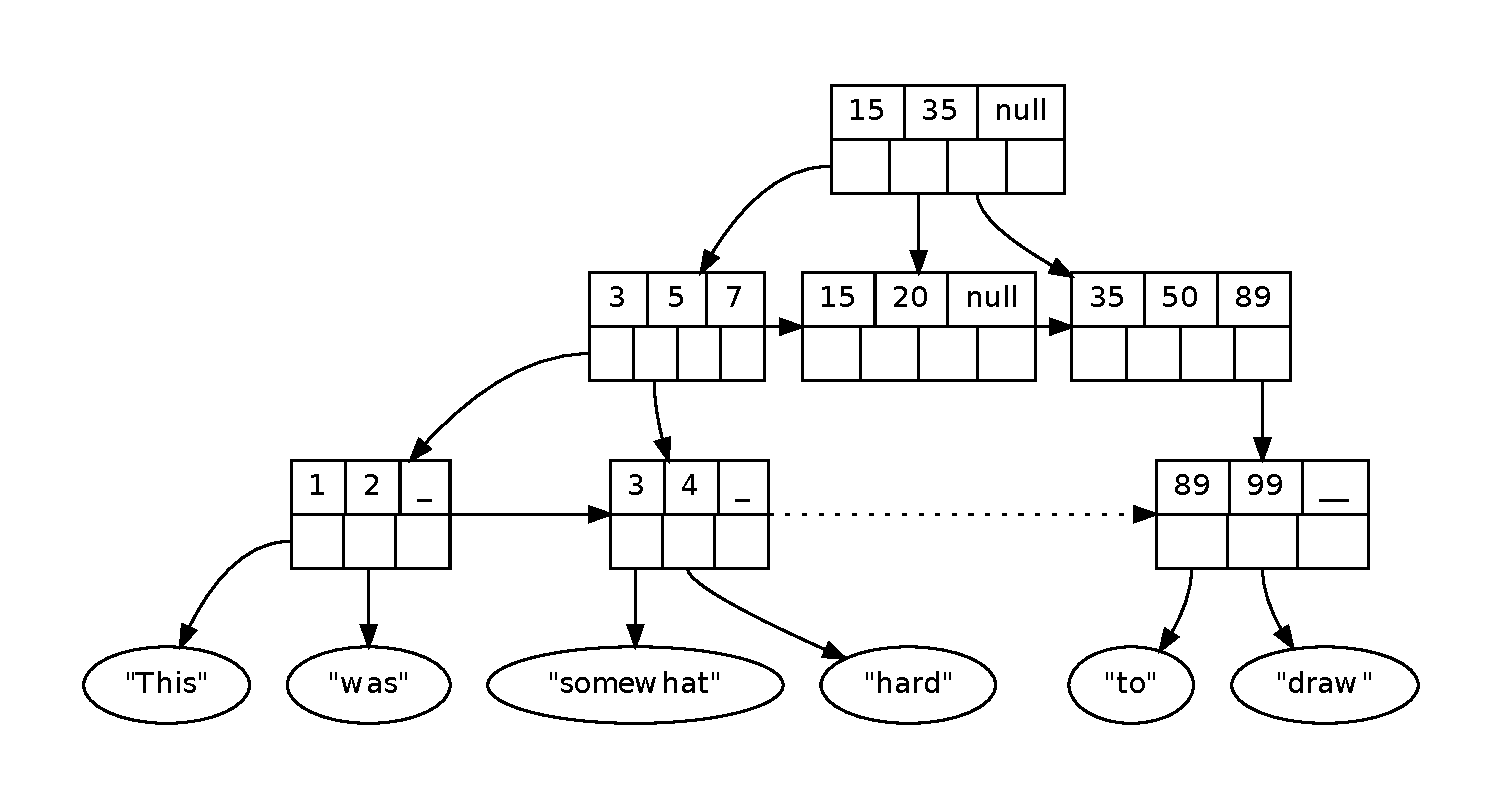
\includegraphics[width=5in]{b_plus_tree_dot.pdf}
\vspace{-1cm}
\end{figure}

    \begin{enumerate}
    \item What Java Collections Framework interface should a
    $\textrm{B}^+$Tree be able to implement?

        \begin{answer}
        \texttt{Java.util.Map$<$K,V$>$}
        \end{answer}
		\vspace{0.125in}

    \item We need to implement two different kinds of nodes for the tree. Why
    do we need to do this? What is different between the two types of nodes?

        \begin{answer}
        Some nodes (the leaves) point to data values. We also have internal
        nodes which point to other nodes (both internal nodes and leaves).
        \end{answer}
		\vspace{0.125in}

    \item We need classes to represent the nodes of the tree. Implement these
    classes so that they use generic types and all of their members are package
    private. Don't implement the constructors or any other methods.

\begin{answer}
\begin{lstlisting}
public interface BTreeNode<K,V> {}

public class InternalNode<K,V> implements BTreeNode<K,V>
{
    K[] keys;
    Node<K,V>[] children;
    InternalNode<K,V> next;
}

public class LeafNode<K,V> implements BTreeNode<K,V>
{
    K keys[];
    V values[];
    LeafNode<K,V> next;
}
\end{lstlisting}
\end{answer}

    \end{enumerate}


\newpage
\item What is the output when \texttt{LookAtDatMagic}'s main is executed?
\begin{lstlisting}
public class HeySteve{
    public int bananza(int in) throws NewException{
        if ( in == 7 ){
            throw new NewException("HeySteve, cut that out!");
        }
        return in;
    }
}

public class NewException extends Exception{
    public NewException(String message){
        super(message);
    }

}
           
public class WakaWaka{
    public String BeachBash(Object a, Object b) throws NewException{
        if ( a.equals(b) ){
            throw new NewException("It's a Beach-bash! WakaWaka!");
        }
        return "Da-nanananan";
    }
}

public class LookAtDatMagic{
    public void magic() throws NewException{
        int maraca = 5;
        try{
            HeySteve steve = new HeySteve();
            maraca = steve.bananza(7);
        }catch(NewException e){
            System.out.println(e.getMessage());
        }finally{
            WakaWaka waka = new WakaWaka();
            System.out.println(waka.BeachBash(maraca, 5));
        }
    }

    public static void main(String[] args){
        try{
            LookAtDatMagic ladm = new LookAtDatMagic();
            ladm.magic();
        }catch(NewException e){
            System.out.println(e.getMessage());
        }
    }
}


\end{lstlisting}
\begin{answer}
HeySteve, cut that out!


It's a Beach-bash! WakaWaka!
\end{answer}
\pagebreak
\item Briefly describe the difference between classes and objects.

    \begin{answer}
    A class is a construct which describes the properties and methods of an
    object. It can be thought of as a mold or template. An object is an 
    instantiation of a class. That is, a specific item created from the class
    ``mold.''
    \end{answer}

\item Briefly describe the difference (for objects) between \texttt{a.equals(b)}, \texttt{a==b},
      \texttt{a.compareTo(b)}, and \texttt{Comparator.compare(a,b)}.

    \begin{answer}
    \begin{itemize}

    \item \texttt{a.equals(b)} Compares objects for equality. Class \texttt{Object} provides a default implementation
	that is overridden for more intelligent behavior.
    Returns a \texttt{boolean}.

    \item \texttt{a == b}  Checks references (if the two objects are the SAME object).
    Can also be used to check whether \texttt{a} is \texttt{null}.

    \item \texttt{a.compareTo(b)} Returns an \texttt{int} indicating whether \texttt{a} is less than (-1),
    equal to (0), or greater than (+1) \texttt{b}, according to their natural ordering.
	Specified by the \texttt{Comparable} interface.

    \item \texttt{compare(a,b)} Returns a negative a $<$ b, 0 if a $=$ b, a positive if a $>$ b. \\
    \texttt{comp1.equals(comp2)} implies that \\ \texttt{sgn(comp1.compare(o1,
    o2))==sgn(comp2.compare(o1, o2))} for every object reference \texttt{o1} and \texttt{o2}.

    \end{itemize}
    \end{answer}

\item Name the design pattern used in the following snippet of code.
\begin{lstlisting}
public class Car
{
	private String make;
	private String model;
	private int mileage;

	private Car(String make, String model, int mileage)
	{
		this.make=make;
		this.model=model;
		this.mileage=mileage;
	}
	public static Car makeCar(String str)
	{
		String arr[] = str.split(" ");
		return new Car(arr[0], arr[1], Integer.parseInteger(arr[2]));
	}

	public static void main(String[] args)
	{
		Car myCar = Car.makeCar("Toyota Camry 200000");
	}
}
\end{lstlisting}

\begin{answer}
The \emph{Factory} design pattern is used.
\vspace{.5in}
\end{answer}
\pagebreak
\item Which layout manager does each of the following descriptions describe?
\begin{enumerate}[(a)]

\item Displays the contained components in a set number of rows and columns,
      where each row has the same height and each column the same width.

\begin{answer}
GridLayout
\vspace{.5in}
\end{answer}

\item Attempts to display the contained components in a single row but will
      create a new row if necessary.

\begin{answer}
FlowLayout
\vspace{.5in}
\end{answer}

\item Allows the developer to specify the region (North, South, East, West,
      Center) of the panel to place the component in.

\begin{answer}
BorderLayout
\vspace{.5in}
\end{answer}

\end{enumerate}

\item 
    \begin{enumerate} 
    \item What is the Java Collections Framework?

    \begin{answer}
        A unified set of interfaces, algorithms and concrete implementations
    provided by Java to support collections of objects
    \end{answer}

    \item Assume the following line of code is given:
    \begin{lstlisting}
        Collection<Integer> t = new ArrayList<Integer>();
    \end{lstlisting}
    What then is wrong with the following? Correct any errors:
    \begin{lstlisting}
        for( int i = 0; i < 20; ++i ){
            t.add(i);
        }
        for( int i=0; i <  t.size(); ++i ){
            System.out.println(t.get(i));
        }
    \end{lstlisting}

    \begin{answer}
    \texttt{Collection} does not support \texttt{get(i)}. The better solution is:
    \begin{lstlisting}
        for( int i = 0; i < 20; ++i ) {
            t.add(i);
        }
        for( Integer i : t ) {
            System.out.println(i);
        }

    \end{lstlisting}
    \end{answer}

    \end{enumerate}
    
\pagebreak
\item Use the following code in this question.

\lstinputlisting{code/ufo/UFO.java}

\pagebreak
\begin{enumerate}
\item Why should \texttt{Probable} be an interface and not a class or an abstract class?

\begin{answer}
\texttt{Probable} needs to define that certain actions can be performed on \texttt{Probable} objects, but does not need to define what those actions should do.
\end{answer}

\item Write the \texttt{Probable} interface.

\begin{answer}
\lstinputlisting{code/ufo/Probable.java}
\end{answer}

\item Should the \texttt{Redneck} and \texttt{Professor} classes implement \texttt{Probable} directly?

\begin{answer}
No!
Since \texttt{Redneck} and \texttt{Professor} objects are stored in variables of type \texttt{Human} they must extend the \texttt{Human} class.
In addition, since the \texttt{Human} variables are able to be added into a collection of \texttt{Probable} objects, the \texttt{Human} class must implement \texttt{Probable}, which will carry down into the \texttt{Redneck} and \texttt{Professor} classes.
\end{answer}

%\end{enumerate}

=======
\end{enumerate}

\section*{Networking}
\item What does TCP stands for? Where and why do we use TCP?

\begin{answer}
Transmission Control Protocol. We use TCP in Telephone Connection because TCP guarantees packet delivery and thus can be considered "lossless and reliable".
\end{answer}

\item What does UDP stands for? When and where do we use UDP?

\begin{answer}
User Datagram Protocol. We use UDP when we are managing a tremendous amount of state (ex: weather data, video transmission).
\end{answer}

\item Which one does a stream socket use for data transmission? TCP (or) UDP?

\begin{answer}
TCP. 
\end{answer}

\item Which one does a datagram socket use for data transmission? TCP (or) UDP?

\begin{answer}
UDP
\end{answer}

\item What is a datagram?

\begin{answer}
independent, self-contained message sent over the network with no guarantees
\end{answer}

\item What is a socket?

\begin{answer}
The endpoints of logical connections between two hosts, which can be used to send and receive data.
\end{answer}

% Networking
\item
	Find at least 3 errors in the following code:

	Server: Echoes one line of data sent to it

	\begin{lstlisting}
ServerSocket pubServer = new ServerSocket(0);
System.out.println(pubServer.getLocalPort());
Socket client;
BufferedReader reader = null;
try {
	reader = new BufferedReader(
		new InputStreamReader(client.getInputStream()));
} catch (IOException e) {
	System.out.println("IOException: " + e.getMessage());
}

String response = null;
try {
	response = reader.readLine();
} catch (IOException e) {
	System.out.println("IOException: " + e.getMessage());
}

System.out.println(response);

pubServer.close();
	\end{lstlisting}

	Client: Sends a line of text to a server: server address, port, text

	\begin{lstlisting}
InetAddress server = null;
try {
	server = InetAddress.getByName(args[0]);
} catch (UnknownHostException e) {
	System.out.println("Unknown host");
}
int port = Integer.parseInt(args[1]);

Socket conn = null;
try {
	conn = new Socket(server, port);
} catch (IOException e) {
	System.out.println("IOException: " + e.getMessage());
}

try {
	System.out.println(args[2]);
} catch (IOException e) {
	System.out.println("IOException: " + e.getMessage());
}

conn.close();
	\end{lstlisting}

	\begin{answer}
		\begin{enumerate}
		\item
			Server: Missing client.close().
		\item
			Server: client never initialized, use pubServer.accept().	
		\item
			Client: Need a PrintWriter writer; writer = new PrintWriter(conn.getOutputStream(), true); writer.println(args[2]); insteand of System.out.println(args[2]);
		\end{enumerate}
	\end{answer}

\end{enumerate}

\end{document}
